\documentclass[10pt,a4paper]{article}
\usepackage[UTF8]{ctex}
\setCJKmainfont[BoldFont=黑体,ItalicFont=楷体]{华文中宋}
\usepackage{amssymb,amsmath,amsfonts,amsthm,mathrsfs,dsfont,graphicx}
\usepackage{ifthen,indentfirst,enumerate,color,titletoc}
\usepackage{tikz}
\usepackage{multicol}
\usepackage{makecell}
\usepackage{longtable}
\usepackage{ifthen}
\usetikzlibrary{arrows,calc,intersections,patterns,decorations.pathreplacing,3d,angles,quotes}
\usepackage[bf,small,indentafter,pagestyles]{titlesec}
\usepackage[top=1in, bottom=1in,left=0.8in,right=0.8in]{geometry}
\renewcommand{\baselinestretch}{2}
\newtheorem{defi}{定义~}
\newtheorem{eg}{例~}
\newtheorem{ex}{~}
\newtheorem{rem}{注~}
\newtheorem{thm}{定理~}
\newtheorem{coro}{推论~}
\newtheorem{axiom}{公理~}
\newtheorem{prop}{性质~}
\newcommand{\blank}[1]{\underline{\hbox to #1pt{}}}
\newcommand{\bracket}[1]{(\hbox to #1pt{})}
\newcommand{\onech}[4]{\par\begin{tabular}{p{.9\textwidth}}
A.~#1\\
B.~#2\\
C.~#3\\
D.~#4
\end{tabular}}
\newcommand{\twoch}[4]{\par\begin{tabular}{p{.46\textwidth}p{.46\textwidth}}
A.~#1& B.~#2\\
C.~#3& D.~#4
\end{tabular}}
\newcommand{\vartwoch}[4]{\par\begin{tabular}{p{.46\textwidth}p{.46\textwidth}}
(1)~#1& (2)~#2\\
(3)~#3& (4)~#4
\end{tabular}}
\newcommand{\fourch}[4]{\par\begin{tabular}{p{.23\textwidth}p{.23\textwidth}p{.23\textwidth}p{.23\textwidth}}
A.~#1 &B.~#2& C.~#3& D.~#4
\end{tabular}}
\newcommand{\varfourch}[4]{\par\begin{tabular}{p{.23\textwidth}p{.23\textwidth}p{.23\textwidth}p{.23\textwidth}}
(1)~#1 &(2)~#2& (3)~#3& (4)~#4
\end{tabular}}
\begin{document}

\begin{enumerate}[1.]

\item 如图, 在平面直角坐标系中, 直线$l_1$与$l_2$垂直, 垂足为$A$, $l_1$、$l_2$与$x$轴的交点分别为$B$、$C$, $\angle ABC=\dfrac \pi 6$. 试分别求直线$l_1$、$l_2$的倾斜角和斜率.
\begin{center}
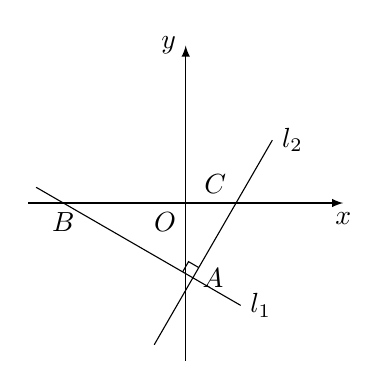
\begin{tikzpicture}[>=latex]
\draw [->, name path = x] (-2,0) -- (2,0) node [below] {$x$};
\draw [->, name path = y] (0,-2) -- (0,2) node [left] {$y$};
\draw (0,0) node [below left] {$O$};
\draw [name path = l1] (-1.9,0.2) --++ (-30:3) node [right] {$l_1$};
\draw [name path = l2] (-0.4,-1.8) --++ (60:3) node [right] {$l_2$};
\draw [name intersections = {of = l1 and l2, by = A}];
\draw [name intersections = {of = l1 and x, by = B}];
\draw [name intersections = {of = l2 and x, by = C}];
\draw (B) node [below] {$B$};
\draw (C) node [above left] {$C$};
\draw (A) node [right] {$A$};
\draw (A) pic [draw, scale = 0.3] {right angle = C--A--B};
\end{tikzpicture}
\end{center}
\item 求经过下列两点的直线的斜率与倾斜角:\\
(1) $P(1, 2)$、$Q(2, -1)$;\\
(2) $M(2, 1)$、$N(a, -2)$, 其中实数$a$是常数.
\item 根据下列直线$l$的倾斜角$\theta$的取值范围, 计算斜率$k$的取值范围:\\
(1) $\theta \in [\dfrac \pi 4, \dfrac \pi 3]$;\\
(2) $\theta \in (\dfrac \pi 2, \dfrac{2\pi} 3)$.
\item 已知三个不同的点$A(2, a)$、$B(a+1, 2a+1)$、$C(-4, 1+a)$在同一条直线上, 求实数$a$的值及该直线的斜率.
\item 如图, 已知点$A(2, 4)$、$B(-1, -1)$、$C(4, 1)$, 过点$B$的直线$l$与线段$AC$相交. 求直线$l$的斜率$k$的取值范围.
\begin{center}
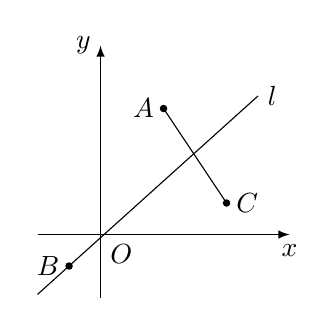
\begin{tikzpicture}[>=latex, scale = 0.4]
\draw [->] (-2,0) -- (6,0) node [below] {$x$};
\draw [->] (0,-2) -- (0,6) node [left] {$y$};
\draw (0,0) node [below right] {$O$};
\filldraw (2,4) circle (0.1) node [left] {$A$} coordinate (A);
\filldraw (-1,-1) circle (0.1) node [left] {$B$} coordinate (B);
\filldraw (4,1) circle (0.1) node [right] {$C$} coordinate (C);
\draw (A) -- (C);
\draw (B) ++ (-1,-0.9) --++ (7,6.3) node [right] {$l$};
\end{tikzpicture}
\end{center}
\item 已知常数$\theta \in [0, \pi)$, 试用$\theta$表示经过$P(0, 0)$、$Q(\sin \theta , \cos \theta)$两点的直线$l$的倾斜角.
\item 设直线$l_1$、$l_2$的倾斜角分别为$\theta_1$、$\theta_2$, 求证: $l_1\perp l_2$的充要条件是$|\theta_1-\theta_2|=\dfrac \pi 2$.
\item 已知直线$l$在平面直角坐标系中的斜率是$k$, 向量$\overrightarrow a$在直线$l$上. 求向量$\overrightarrow a$在$x$轴上的投影向量.
\item 已知直线$l$经过点$P(3, 5)$, 倾斜角为$\alpha$且$\cos\alpha=\dfrac 35$. 求直线$l$的点斜式方程.
\item 已知直线$l$在$y$轴上的截距为$4$, 倾斜角为$\alpha$且$\sin\alpha=\dfrac 35$. 求直线$l$的斜截式方程.
\item 求下列直线的斜率与在$x$、$y$两坐标轴上的截距:\\
(1) $l_1: y+1=-\dfrac {\sqrt 3}3(x+1)$;\\
(2) $l_2: y=-3x+\sqrt 3$.
\item 已知直线$l: y=kx+2$经过点$(1, -3)$.\\
(1) 求$l$的倾斜角的大小;\\
(2) 求$l$在$x$轴上的截距.
\item 直线$l$经过点$P(-2, 1)$, 在$x$轴、$y$轴上的截距分别为$a$、$b$. 已知$a+b=4$, 求直线$l$的方程.
\item 根据给定条件, 求下列直线的两点式方程:\\
(1) 直线$l_1$经过点$A(2, 0)$、$B(3, 7)$;\\
(2) 直线$l_2$与坐标轴的交点分别为$(3, 0)$、$(0, -1)$.
\item 已知$\triangle ABC$的三个顶点的坐标分别为$A(3, 8)$、$B(3, -2)$、$C(-3, 0)$.\\
(1)求边$BC$所在直线的方程;\\
(2)求边$BC$上的中线所在直线的方程.
\item 设直线$l$在$x$轴与$y$轴上的截距分别是$a$与$b$, 且$a$与$b$均不为零. 求证: 直线$l$的方程可以写成$\dfrac xa+\dfrac yb=1$.
\item 一个弹簧在弹性限度内挂$4\text{kg}$的物体时弹簧长度为$20\text{cm}$, 挂$5\text{kg}$物体时弹簧长度为$21.5\text{cm}$. 已知在弹性限度内所挂物体的质量$x$(单位: $\text{kg}$)与弹簧长度$y$(单位: $\text{cm}$)的关系可以用直线的方程表示, 求该直线的方程, 并求弹簧自身的长度.
\item 在平面直角坐标系中, 作出下列直线, 并求它们的斜率与倾斜角.\\
(1) $l_1: 3x-y-2=0$;\\
(2) $l_2: 3x+2y-1=0$.
\item 设直线$l$的方程是$ax+by+c=0$, 在下列条件下, 求实数$a$、$b$、$c$满足的条件:\\
(1) $l$与$x$轴、$y$轴均相交;\\
(2) $l$经过第二、第三、第四象限.
\item 已知直线$l: ax+(4-2a)y-3=0$, 根据下列条件, 求实数$a$的值:\\
(1) $l$经过点$(1, 1)$;\\
(2) $l$在两个坐标轴上的截距相等.
\item 已知$A(7, -4)$、$B(-5, 6)$两点, 求线段$AB$的垂直平分线的点法式方程.
\item 已知直线$l_1: 3kx+(k+2)y+6=0$, 直线$l_2: kx+(2k-3)y+2=0$. 若这两条直线的法向量互相垂直, 求$k$的值.
\item 已知平行四边形$ABCD$中, 三个顶点的坐标分别为$A(1, 2)$、$B(3, 4)$、$C(2, 6)$.分别求边$AD$、$CD$所在直线的方程.
\item 已知直线$l$经过点$P(2, -1)$, 与$x$轴、$y$轴分别交于$A$、$B$两点. 若$2\overrightarrow{PA}+\overrightarrow{PB}=\overrightarrow 0$, 求直线$l$的方程.
\item 直线$l: y=kx+b$($k$、$b\in \mathbf{R}$)与线段$AB$相交, 其中点$A$为$(4, 2)$, 点$B$为$(1, 5)$.\\
(1) 当$b=-1$时, 求$k$的取值范围;\\
(2) 当$k=1$时, 求$b$的取值范围.
\item 已知$\triangle ABC$中, 两个顶点的坐标分别为$A(-2, 1)$、$B(4, -3)$, 点$G(0, 2)$是此三角形的重心. 求边$BC$、$AC$所在直线的方程.
\item 若$2x_1+3y_1=1, 2x_2+3y_2=1$, 且$x_1\ne x_2$. 求经过两点$A(x_1, y_1)$、$B(x_2, y_2)$的直线$l$的方程.
\item 如图是一个$\text{W}$形的霓虹灯(灯管宽度忽略不计), 每边长都是$2\text{m}$, 每相邻两边相交所成的锐角都是$30^\circ$. 试建立适当的平面直角坐标系, 写出此霓虹灯的每条边所在直线在这个坐标系中的方程.
\begin{center}

\begin{tikzpicture}[>=latex]
\draw [very thick] (0,0) --++ (-75:2) --++ (75:2) --++ (-75:2) --++ (75:2);
\end{tikzpicture}
\end{center}
\item 证明: 直线$2x+(1-\cos 2\theta)y-\sin \theta =0$($\theta \in \mathbf{R}$且不是$\pi$的整数倍)和两坐标轴围成图形的面积是定值.
\item 已知直线$l: (a-1)x+(3-2a)y+a+1=0$.\\
(1) 若直线的斜率$k\in [-1, 2]$, 求实数$a$的取值范围;\\
(2) 求证:对任意实数$a$, 直线$l$都经过一个定点.
\item 根据下列方程, 判定直线$l_1$与$l_2$的位置关系:\\
(1)$l_1: 2x-3y-1=0$, $l_2: 4x-6y-2=0$;\\
(2)$l_1: y=\dfrac 13x+1$, $l_2: x-6y-2=0$;\\
(3)$l_1: (\sqrt 5-1)x-2y+1=0$, $l_2: 2x-(\sqrt 5-1)y-2=0$.
\item 已知直线$l_1: 6x+(t-1)y-8=0$, 直线$l_2: (t+4)$x+$(t+6)y-16=0$. 根据下列条件, 求实数$t$的取值范围:\\
(1) $l_1$与$l_2$相交;\\
(2) $l_1\parallel l_2$;\\
(3) $l_1$与$l_2$重合.
\item 已知两条直线$l_1: (t-1)x+2y-t=0$和$l_2: $$x+ty+t-2=0$, 且$l_1\parallel l_2$. 求实数$t$的值.
\item 已知平行四边形$ABCD$中, 一组对边$AB$、$CD$所在直线的方程分别为$ax+4y=a+2$, $x+ay=a$. 求实数$a$的值.
\item 已知四边形$ABCD$的四个顶点的坐标分别为$A(-1, 2)$、$B(3, 4)$、$C(3, 2)$、$D(1, 1)$, 求证:四边形$ABCD$是梯形.
\item 已知直线$l_1: (k-3)x+(5-k)y+1=0$与直线$l_2: 2(k-3)x-2y+(2-k)=0$互相垂直, 求实数$k$的值.
\item 已知直线$l$垂直于直线$l': 2x+3y-4=0$, 根据下列条件求$l$的方程:\\
(1) $l$经过点$(1, 1)$;\\
(2) $l$与坐标轴围成的三角形的面积是$3$.
\item 已知等腰直角三角形$ABC$的斜边$AB$所在直线的方程为$3x-y-5=0$, 直角顶点为$C(4, -1)$. 求两条直角边所在直线的方程.
\item 根据下列方程, 求直线$l_1$与$l_2$的夹角的大小:\\
(1) $l_1: x+3y+2=0$, $l_2: 4x+2y-1=0$;\\
(2) $l_1: x+2y-3=0$, $l_2: x-y-5=0$;\\
(3) $l_1: 2x-3y+6=0$, $l_2: x-5=0$.
\item 若直线$x+my+5=0$与直线$x+y+1=0$的夹角为$\pi 4$, 求实数$m$的值.
\item 已知等腰直角三角形$ABC$的直角边$BC$所在直线的方程为$x-2y-6=0$, 顶点$A$的坐标为$(0, 6)$. 分别求直角边$AC$、斜边$AB$所在直线的方程.
\item 给定直线$l_1: y=ax+b$, 直线$l_2: y=bx-a$. 已知直线$l_1$的倾斜角为$\dfrac{3\pi} 4$, 且它与直线$l_2$的交点落在直线$l_3: 2x+y-2=0$上. 求实数$b$的值.
\item 求证:不论实数$\lambda$取何值, 直线$l: 2x+y-4+\lambda (x-y+2)=0$经过同一个点, 并求所有这些直线的公共点.
\item 已知集合$A=\{(x, y)|2x-(a+1)y-1=0\}$, $B=\{(x, y)|ax-y+1=0\}$, 且$A\cap B=\varnothing$. 求实数$a$的值.
\item 分别求经过直线$l_1: 5x+2y-3=0$和$l_2: $$3x-5y-8=0$的交点, 且与直线$x+4y-7=0$垂直、平行的直线的方程.
\item 已知$\triangle ABC$的一个顶点为$A(3, -4)$, 有两条高所在直线的方程分别是$7x-2y-1=0$与$2x-7y-6=0$. 求$\triangle ABC$三条边所在直线的方程.
\item 求直线$l_1: x+y-3=0$与直线$l_2: 7x-y-5=0$夹角平分线的方程.
\item 一束光线经过点$(-2, 1)$, 由直线$l: y=x$反射后, 经过点$(3, 5)$射出. 求反射光线所在直线的方程.
\item 求点$P(2, 3)$到直线$l$的距离:\\
(1) $l: 3x-2y=13$;\\
(2) $l: y=-2x+3$.
\item 已知点$A(a, 6)$到直线$3x-4y-4=0$的距离等于$4$, 求实数$a$的值.
\item 求下列两条平行线之间的距离:\\
(1) $l_1: 2x-3y+1=0$, $l_2: 4x-6y+1=0$;\\
(2) $l_1: y=\dfrac{\sqrt 3}2x+1$, $l_2: \sqrt 3x-2y+1=0$.
\item 已知直线$l_1: 2x-y+a=0$与直线$l_2: -4x+2y+1=0$的距离为$\dfrac{7\sqrt 5}{10}$, 求实数$a$的值.
\item 已知点$A(1, 0)$、$B(4, -4)$. 若点$A$与点$B$到直线$l$的距离都为$2$, 求直线$l$的方程. 
\item 已知点$P$是直线$3x-4y+2=0$上任意一点, 求点$P$与点$A(3, -1)$之间距离的最小值.
\item 已知直线$l$经过点$P(1, 1)$且与直线$l_1: y=\sqrt 3x+1$和$l_2: y=\sqrt 3x+3$分别交于点$A$和点$B$. 若$|AB|=\sqrt 2$, 求直线$l$的方程.
\item 根据下列条件, 分别求圆的方程:\\
(1) 圆心为$C(-\dfrac 32, 3)$, 半径$r=\sqrt 3$;\\
(2) 圆心为$C(\sqrt 2, 1)$, 过点$A(-1, \sqrt 2)$;\\
(3) 与$x$轴相交于$A(1, 0)$、$B(5, 0)$两点, 且半径等于$\sqrt 5$.
\item 已知圆$(x-a)^2+(y-b)^2=r^2$($r>0$), 求在下列情况下, 实数$a$、$b$、$r$应分别满足什么条件:\\
(1) 圆过原点;\\
(2) 圆心在$x$轴上;\\
(3) 圆与$x$轴相切;\\
(4) 圆与两坐标轴均相切.
\item 求过点$M(5, 2)$、$N(3, 2)$, 且圆心在直线$y=2x-3$上的圆的方程.
\item 已知$a^2x^2+(a+2)y^2+2ax+a=0$表示圆, 求实数$a$的值.
\item 直线$l$与圆$x^2+y^2+2x-4y+a=0$($a<3$)相交于$A$、$B$两点, 且弦$AB$的中点为$(0, 1)$. 求直线$l$的方程.
\item 已知圆过原点, 且与$x$轴、$y$轴的交点的坐标分别为$(a, 0)$、$(0, b)$, 其中$ab\ne 0$.求这个圆的方程.
\item 判断直线$x\cos \theta +y\sin \theta =r$与圆$x^2+y^2=r^2$的位置关系.
\item 已知直线$2x+3y+1=0$和圆$x^2+y^2-2x-3=0$相交于$A$、$B$两点, 求弦$AB$的垂直平分线的方程.
\item 求与圆$x^2+y^2=25$内切于点$P(3, -4)$且半径为$1$的圆的方程.
\item 已知圆$C$过点$(-4, 0)$且与圆$x^2+y^2-4x-6y=0$相切于原点, 求圆$C$的方程.
\item 圆拱桥的一个圆拱如图所示, 该圆拱的跨度$AB$为$20\text{m}$, 拱高$OP$为$4\text{m}$, 在建造过程中每隔$4\text{m}$需用一个支柱支撑. 求支柱$A_2B_2$的高度. (结果精确到$0.01\text{m}$)
\begin{center}
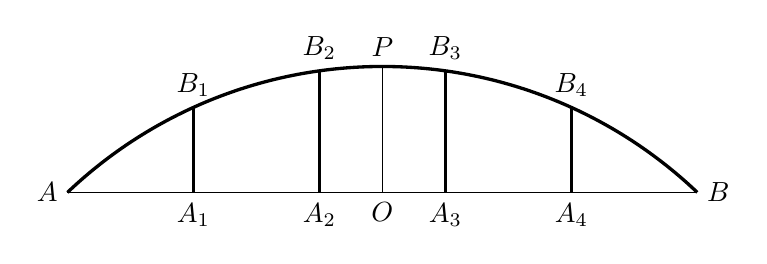
\begin{tikzpicture}[>=latex,scale = 0.4]
\draw [domain = -10:10, samples= 200, very thick] plot (\x,{sqrt(210.25-pow(\x,2))-10.5});
\draw (-10,0) node [left] {$A$} -- (10,0) node [right] {$B$};
\draw (0,0) node [below] {$O$} -- (0,4) node [above] {$P$};
\draw [very thick](-6,0) node [below] {$A_1$} -- (-6,{sqrt(210.25-pow(6,2))-10.5}) node [above] {$B_1$};
\draw [very thick](-2,0) node [below] {$A_2$} -- (-2,{sqrt(210.25-pow(2,2))-10.5}) node [above] {$B_2$};
\draw [very thick](2,0) node [below] {$A_3$} -- (2,{sqrt(210.25-pow(2,2))-10.5}) node [above] {$B_3$};
\draw [very thick](6,0) node [below] {$A_4$} -- (6,{sqrt(210.25-pow(6,2))-10.5}) node [above] {$B_4$};
\end{tikzpicture}
\end{center}
\item 给定点$A(2, 3)$与圆$C: x^2+y^2=25$, 求圆$C$的过点$A$最短弦所在直线的方程.
\item 一个圆过点$(2, -1)$, 圆心在直线$2x+y=0$上, 且与直线$x-y-1=0$相切. 求这个圆的方程.
\item 已知圆$x^2+y^2+6x-8y+25=r^2$与$x$轴相切, 求这个圆截$y$轴所得的弦长.
\item 求圆$C: x^2+y^2+4x+2y-3=0$关于点$M(1, 1)$对称的圆的方程.
\item 已知动直线$kx-y+1=0$(其中$k\in \mathbf{R}$)和圆$x^2+y^2=4$相交于$A$、$B$两点, 求弦$AB$的中点的轨迹方程.
\item 求经过点$(5, -5)$且与圆$x^2+y^2=25$相切的直线的方程.
\item 已知直线$y=x+m$和曲线$y=\sqrt{1-x^2}$有两个不同的交点, 求实数$m$的取值范围.
\item 已知直线$l: x-y+4=0$与圆$C: (x-1)^2+(y-1)^2=2$, 求圆$C$上各点到直线$l$的距离的最大值.
\item 已知实数$x$、$y$满足$(x-2)^2+y^2=3$, 求$\dfrac yx$的取值范围.
\item $400\text{m}$标准跑道的内圈如图所示($400\text{m}$标准跑道最内圈的长度为$400\text{m}$), 其中左右两端均是半径为$36\text{m}$的半圆弧.
\begin{center}
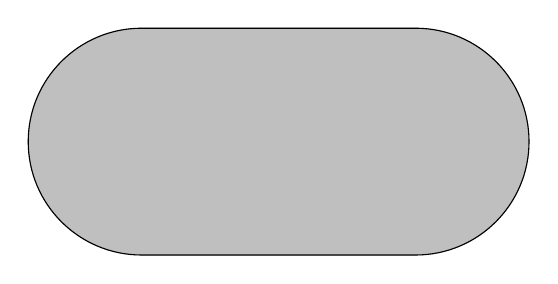
\begin{tikzpicture}[>=latex,scale = 0.4]
\filldraw [gray!50] (0,0) -- (8.7,0) arc (-90:90:3.6) --++ (-8.7,0) arc (90:270:3.6) -- cycle; 
\draw (0,0) -- (8.7,0) arc (-90:90:3.6) --++ (-8.7,0) arc (90:270:3.6); 
\end{tikzpicture}
\end{center}
(1) 求每条直道的长度; ($\pi$取$3.14$, 结果精确到$1\text{m}$)\\
(2) 建立适当的平面直角坐标系, 写出上半部分跑道所对应的函数表达式.
\item 若方程$16x^2+ky^2=16k$表示焦点在$y$轴上的椭圆, 求实数$k$的取值范围.
\item 设$F$是椭圆的一个焦点, $B_1B_2$是椭圆的短轴, $\angle  B_1FB_2=60^\circ$. 求椭圆的离心率.
\item 已知椭圆的一个焦点是$F_1(-3, 0)$, 且经过点$P(2, \sqrt 2)$. 求这个椭圆的标准方程.
\item 直线$y=2x+b$被椭圆$4x^2+y^2=16$所截得的弦长为$\sqrt{35}$, 求实数$b$的值.
\item 若对于任意实数$k$, 直线$y=kx+1$与椭圆$\dfrac{x^2}5+\dfrac{y^2}m=1$恒有公共点. 求实数$m$的取值范围.
\item 已知$P$是椭圆$\dfrac{x^2}{25}+\dfrac{y^2}9=1$上的点, $F_1$、$F_2$是椭圆的两个焦点.\\
(1) 若$\angle F_1PF_2=60^\circ$, 求$\triangle PF_1F_2$的面积;\\
(2) 若$\triangle PF_1F_2$的面积为$9$, 求$\angle F_1PF_2$的大小.
\item 水星的运行轨道是以太阳的中心为一个焦点的椭圆, 轨道上离太阳中心最近的距离约为$4.7\times 10^8\text{km}$, 最远的距离约为$7.05\times 10^8\text{km}$. 以这个轨道的中心为原点, 以太阳中心及轨道中心所在直线为$x$轴, 建立平面直角坐标系. 求水星运行轨道的方程. (长半轴的长和短半轴的长精确到$0. 1\times 10^8\text{km}$)
\item 双曲线$\dfrac{x^2}{64}-\dfrac{y^2}{36}=1$上一点$P$到焦点$F_1$的距离等于$6$, 求点$P$到另一焦点$F_2$的距离.
\item 已知双曲线以坐标轴为对称轴, 两个顶点间的距离为$2$, 焦点到渐近线的距离为$\sqrt 2$. 求该双曲线的方程.
\item 如果双曲线关于原点对称, 它的焦点在坐标轴上, 实轴的长为$8$, 焦距为$10$. 写出此双曲线的方程.
\item 如果方程$\dfrac{x^2}{m+2}-\dfrac{y^2}{m+1}=1$表示焦点在$y$轴上的双曲线, 求实数$m$的取值范围.
\item 已知双曲线经过点$(1, 1)$, 其渐近线方程为$y=\pm\sqrt 2x$. 求此双曲线的方程.
\item 已知双曲线的中心在原点, 焦点在$y$轴上, 并且双曲线上两点$P_1$、$P_2$的坐标分别为$(3, -4\sqrt 2)$、$(\dfrac 94, 5)$. 求该双曲线的方程.
\item 已知离心率为$\dfrac 53$的双曲线与椭圆$\dfrac{x^2}{40}+\dfrac{y^2}{15}=1$有公共焦点, 求此双曲线的方程.
\item $A$、$B$、$C$是我方三个炮兵阵地. $A$地在$B$地的正东, 相距$6\text{km}$; $C$地在$B$地的北偏西$30^\circ$, 相距$4\text{km}$. $P$为敌方炮兵阵地. 某时刻$A$地发现$P$地某种信号, $12\text{s}$后$B$、$C$两地才同时发现这种信号(该信号的传播速度为$0. 333\text{km}$/$\text{s}$). 若从$A$地炮击$P$地, 求准确炮击的方位角. (结果精确到$1^\circ$)
\item 求抛物线$y^2=ax$($a\ne 0$)的焦点坐标和准线方程.
\item 若抛物线$y^2=2x$上的$A$、$B$两点到焦点$F$的距离之和是$5$, 求线段$AB$的中点的横坐标.
\item 求以坐标原点为顶点, 以$y$轴为对称轴, 并经过点$P(-6, -3)$的抛物线的标准方程.
\item 已知直线$y=kx-4$与抛物线$y^2=8x$有且只有一个公共点, 求实数$k$的值.
\item 已知一隧道的顶部是抛物拱形, 拱高是$5\text{m}$, 跨度为$10\text{m}$. 建立适当的平面直角坐标系, 求此拱形所在的抛物线方程.
\item 已知动点$P$与定点$(1, 0)$的距离比点$P$到$y$轴的距离大$1$, 求动点$P$的轨迹方程.
\item 过抛物线$y^2=2px$($p>0$)焦点的一条直线与抛物线相交于两个不同的点, 求证: 这两个点的纵坐标$y_1$、$y_2$满足$y_1y_2=-p^2$.
\item 过抛物线$y^2=2px$的焦点且倾斜角为$\alpha$的直线$l$与抛物线交于$A$、$B$两点, 求证:$|AB|=\dfrac{2p}{\sin^2\alpha}$.
\item 写出椭圆方程推导过程中的``反过来推演'', 即验证:若点$M$以方程$\dfrac{x^2}{a^2}+\dfrac{y^2}{b^2}=1$($a>b>0$)的解$(x, y)$为坐标, 则点$M$一定在以$F_1(-c, 0)$与$F_2(c, 0)$为焦点的椭圆上, 这里$c=\sqrt{a^2-b^2}$.
\item 给定$A(-3, 2)$、$B(3, -2)$两点, 求证:与这两点距离相等的点$P$的轨迹方程是$3x-2y=0$.
\item 已知点$P(2, 1)$在方程$x^2+k^2y^2-3x-ky-4=0$所表示的曲线上, 求实数$k$的值.
\item 定长为$4$的线段$AB$的两端点分别在$x$轴、$y$轴上滑动, 求$AB$中点的轨迹方程.
\item 已知动点$C$到点$A(2, 0)$的距离是它到点$B(8, 0)$的距离的一半, 求点$C$的轨迹方程.
\item 证明:到两坐标轴距离相等的点的轨迹方程是$x^2-y^2=0$.
\item 已知曲线$C: y^2=x+1$和定点$A(3, 1)$, 点$B$在曲线$C$上运动. 求满足$\overrightarrow{AP}=2\overrightarrow{PB}$的点$P$的轨迹方程.
\item 求过点$M(2, \dfrac \pi 2)$且平行于极轴的直线的极坐标方程.
\item 求极坐标方程分别是$\rho=2\cos \theta$和$\rho=2\sin \theta$的两个圆的圆心距.
\item 作出下列方程的曲线:\\
(1) $x^2-y^2=0$;\\
(2) $x^2+2xy-3y^2=0$.
\item 已知圆$x^2+y^2-2x+2y-3=0$和圆$x^2+y^2+4x-1=0$关于直线$l$对称, 求直线$l$的方程.
\item 证明:椭圆$C_1: \dfrac{x^2}4+\dfrac{y^2}3=1$与椭圆$C_2: \dfrac{x^2}3+\dfrac{y^2}4=1$的四个交点共圆.
\item 点$P$在椭圆$\dfrac{x^2}4+y^2=1$上运动, 求它到直线$l: x+2y-2=0$的距离的最大值.
\item 点$P$到定点$F(2, 0)$的距离与它到直线$x=8$的距离之比为$k$, 请分别给出$k$的某个值, 使得轨迹是椭圆、双曲线和抛物线.
\item 已知椭圆$C: \dfrac{x^2}4+\dfrac{y^2}3=1$, 试确定$m$的取值范围, 使该椭圆上有两个不同的点关于直线$l: y=4x+m$对称.
\item 在极坐标系中, 求曲线$\rho=\cos \theta +1$与$\rho \cos \theta =1$的公共点到极点的距离.
\item 在长方体$ABCD-A'B'C'D'$中, $|AB|=4$, $|BC|=3$, $|AA'|=5$. 写出:\\(1) 与$\overrightarrow{AC'}$有相等模的向量;\\
(2) $\overrightarrow{AB}$的相等向量;\\
(3) 与$\overrightarrow{AA'}$垂直的向量.
\item 如图, 在直三棱柱$ABC-A_1B_1C_1$中, $\overrightarrow{CA}=\overrightarrow a$, $\overrightarrow{CB}=\overrightarrow b$, $\overrightarrow{CC_1}=\overrightarrow c$. 将向量$\overrightarrow{A_1B}$表示为$\overrightarrow a$、$\overrightarrow b$、$\overrightarrow c$的线性组合.
\begin{center}
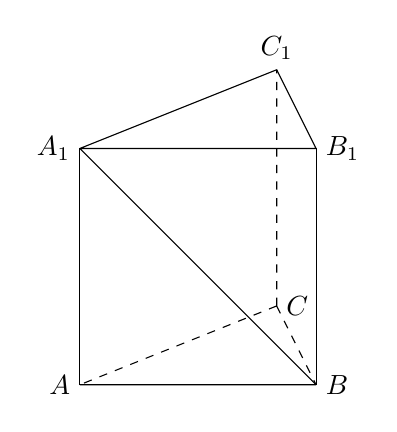
\begin{tikzpicture}[>=latex]
\draw (0,0) node [left] {$A$} coordinate (A);
\draw (3,0) node [right] {$B$} coordinate (B);
\draw (1.5,0,0) ++ (0,0,{-1.5*sqrt(3)}) node [right] {$C$} coordinate (C);
\draw (A) --++ (0,3) node [left] {$A_1$} coordinate (A1);
\draw (B) --++ (0,3) node [right] {$B_1$} coordinate (B1);
\draw (C) ++ (0,3) node [above] {$C_1$} coordinate (C1);
\draw [dashed] (C) -- (A) (C) -- (B) (C) -- (C1);
\draw (A) -- (B) (A1) -- (B1) (C1) -- (A1) (C1) -- (B1) (A1) -- (B);
\end{tikzpicture}
\end{center}
\item 如图, 在正方体$ABCD-A'B'C'D'$中, $E$是$A'C'$的中点, 点$F$在$AE$上, 且$|AF|=\dfrac 12|EF|$. 试用向量$\overrightarrow{AA'}$、$\overrightarrow{AB}$与$\overrightarrow{AD}$的线性组合表示$\overrightarrow{AF}$.
\begin{center}
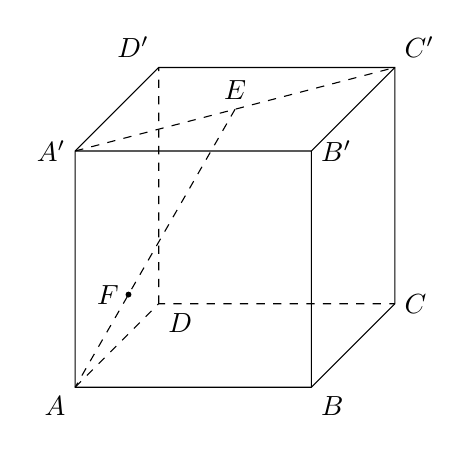
\begin{tikzpicture}[>=latex]
\draw (0,0) node [below left] {$A$} coordinate (A) --++ (3,0) node [below right] {$B$} coordinate (B) --++ (45:{3/2}) node [right] {$C$} coordinate (C)
--++ (0,3) node [above right] {$C'$} coordinate (C1)
--++ (-3,0) node [above left] {$D'$} coordinate (D1) --++ (225:{3/2}) node [left] {$A'$} coordinate (A1) -- cycle;
\draw (A) ++ (3,3) node [right] {$B'$} coordinate (B1) -- (B) (B1) --++ (45:{3/2}) (B1) --++ (-3,0);
\draw [dashed] (A) --++ (45:{3/2}) node [below right] {$D$} coordinate (D) --++ (3,0) (D) --++ (0,3);
\draw [dashed] (A1) -- (C1);
\draw ($(A1)!0.5!(C1)$) node [above] {$E$} coordinate (E);
\draw [dashed] (E) -- (A);
\filldraw ($(A)!{1/3}!(E)$) circle (0.03) node [left] {$F$} coordinate (F); 
\end{tikzpicture}
\end{center}
\item 已知$\overrightarrow a\perp \overrightarrow b$, $\overrightarrow c$与$\overrightarrow a$、$\overrightarrow b$的夹角都是$60^\circ$, 且$|\overrightarrow a|=1$, $|\overrightarrow b|=2$, $|\overrightarrow c|=3$. 计算:\\
(1) $(3\overrightarrow a-2\overrightarrow b)\cdot (\overrightarrow b-3\overrightarrow c)$;\\
(2) $|\overrightarrow a+2\overrightarrow b-\overrightarrow c|$.
\item 已知空间四边形$ABCD$中, $AB\perp CD, AC\perp BD$. 求证: $AD\perp BC$.
\item 如图, 在四面体$ABCD$中, $E$、$M$、$N$分别是棱$AB$、$AC$、$AD$的中点, $E_1$、$M_1$、$N_1$分别是棱$CD$、$BD$、$BC$的中点, $G$是线段$EE_1$的中点. 试判断下列各组中的三点是否共线:
\begin{center}
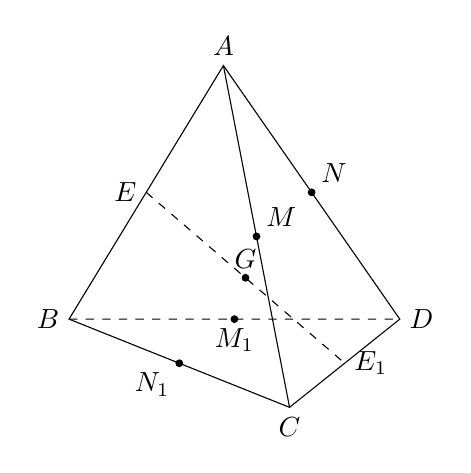
\begin{tikzpicture}[>=latex,scale = 1.4]
\draw (0,0) node [left] {$B$} coordinate (B);
\draw (3,0) node [right] {$D$} coordinate (D);
\draw (1.4,2.3) node [above] {$A$} coordinate (A);
\draw (2,-0.8) node [below] {$C$} coordinate (C);
\draw ($(A)!0.5!(B)$) node [left] {$E$} coordinate (E);
\draw ($(D)!0.5!(C)$) node [right] {$E_1$} coordinate (E1);
\filldraw ($(A)!0.5!(C)$) circle (0.03) node [above right] {$M$} coordinate (M);
\filldraw ($(A)!0.5!(D)$) circle (0.03) node [above right] {$N$} coordinate (N);
\filldraw ($(B)!0.5!(C)$) circle (0.03) node [below left] {$N_1$} coordinate (N1);
\filldraw ($(B)!0.5!(D)$) circle (0.03) node [below] {$M_1$} coordinate (M1);
\filldraw ($(E)!0.5!(E1)$) circle (0.03) node [above] {$G$} coordinate (G);
\draw (A) -- (B) -- (C) -- (D) -- cycle;
\draw (A) -- (C);
\draw [dashed] (E) -- (E1) (B) -- (D);
\end{tikzpicture}
\end{center}
(1) $G$、$M$、$M_1$;\\
(2) $G$、$N$、$N_1$.
\item 如图, $A$是$\triangle BCD$所在平面外一点, $G$是$\triangle BCD$的重心.求证: $\overrightarrow{AG}=\dfrac 13(\overrightarrow{AB}+\overrightarrow{AC}+\overrightarrow{AD})$.
\begin{center}
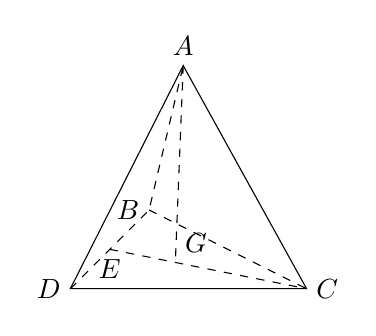
\begin{tikzpicture}[>=latex]
\draw (0,0) node [left] {$D$} coordinate (D);
\draw (3,0) node [right] {$C$} coordinate (C);
\draw (1,1) node [left] {$B$} coordinate (B);
\draw ($(B)!0.5!(D)$) node [below] {$E$} coordinate (E);
\draw ($(E)!{1/3}!(C)$) node [above right] {$G$} coordinate (G);
\draw (G) ++ (0.1,2.5) node [above] {$A$} coordinate (A);
\draw (A) -- (D) -- (C) -- cycle;
\draw [dashed] (A) -- (G) (D) -- (B) -- (A) (B) -- (C) (E) -- (C);
\end{tikzpicture}
\end{center}
\item 如图, 在三棱锥$D-ABC$中, $\angle DAC=\angle BAC=60^\circ$, $AC=1$, $AB=2$, $AD=3$.\\
(1) 求$\overrightarrow{AC}\cdot \overrightarrow{BD}$, 并说明异面直线$AC$与$BD$所成的角$\theta$的大小在棱$BD$长度增大时是怎样变化的;\\
(2) 若$AC\perp BC$, 判断点$D$在平面$ABC$上的射影是否可能在直线$BC$上, 给出你的结论并加以证明.
\begin{center}
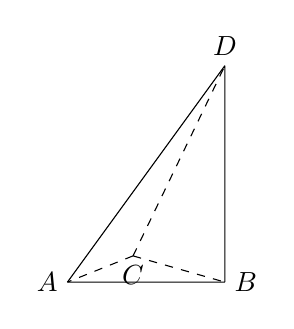
\begin{tikzpicture}[>=latex]
\draw (0,0,0) node [left] {$A$} coordinate (A);
\draw (2,0,0) node [right] {$B$} coordinate (B);
\draw (0.5,0,{-0.5*sqrt(3)}) node [below] {$C$} coordinate (C);
\draw ({3/2},{9/4},{-3*sqrt(3)/4}) node [above] {$D$} coordinate (D);
\draw (A) -- (B) (A) -- (D) (B) -- (D);
\draw [dashed] (C) -- (A) (C) -- (B) (C) -- (D);
\end{tikzpicture}
\end{center}
\item 在空间中还可以讨论一个向量$\overrightarrow{AB}$在一个平面$\alpha$上的投影. 如图, 若$\overrightarrow a=\overrightarrow{AB}$, 点$A$与点$B$在平面$\alpha$上的投影分别是点$A'$与点$B'$, 则$\overrightarrow a=\overrightarrow{AB}$在平面$\alpha$上的投影就是向量$\overrightarrow{A'B'}$. 现在给定向量$\overrightarrow a$、平面$\alpha$以及平面$\alpha$上的非零向量$\overrightarrow b$. 设向量$\overrightarrow a$在平面$\alpha$上的投影是向量$\overrightarrow{a'}$, 向量$\overrightarrow{a'}$在向量$\overrightarrow b$方向上的投影是向量$\overrightarrow{a''}$. 求证:向量$\overrightarrow{a''}$是向量$\overrightarrow a$在向量$\overrightarrow b$方向上的投影.
\begin{center}
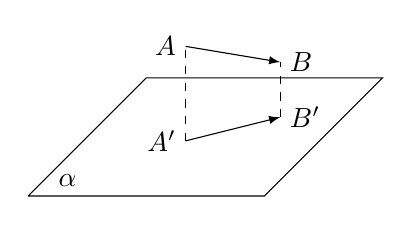
\begin{tikzpicture}[>=latex]
\draw (0,0) -- (3,0) --++ (1.5,1.5) --++ (-3,0) -- (0,0) ++ (0.5,0) node [above] {$\alpha$};
\draw [->] (2,0.7) node [left] {$A'$} -- (3.2,1) node [right] {$B'$};
\draw [->] (2,1.9) node [left] {$A$} -- (3.2,1.7) node [right] {$B$};
\draw [dashed] (2,0.7) -- (2,1.9) (3.2,1) -- (3.2,1.7);
\end{tikzpicture}
\end{center}
\item 如图, 在平行六面体$ABCD-A_1B_1C_1D_1$中, 设$\overrightarrow{D_1A}=\overrightarrow a$, $\overrightarrow{D_1B_1}=\overrightarrow b$, $\overrightarrow{D_1C}=\overrightarrow c$. 试用$\overrightarrow a$、$\overrightarrow b$、$\overrightarrow c$表示$\overrightarrow{D_1B}$.
\begin{center}
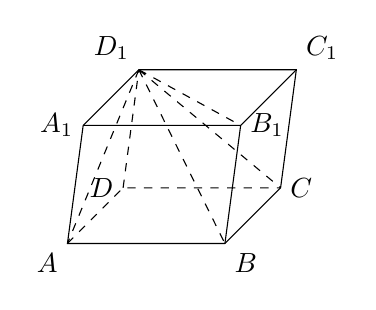
\begin{tikzpicture}[>=latex]
\draw (0,0) node [below left] {$A$} coordinate (A) --++ (2,0) node [below right] {$B$} coordinate (B) --++ (45:{2/2}) node [right] {$C$} coordinate (C)
--++ (0.2,1.5) node [above right] {$C_1$} coordinate (C1)
--++ (-2,0) node [above left] {$D_1$} coordinate (D1) --++ (225:{2/2}) node [left] {$A_1$} coordinate (A1) -- cycle;
\draw (A) ++ (2.2,1.5) node [right] {$B_1$} coordinate (B1) -- (B) (B1) --++ (45:{2/2}) (B1) --++ (-2,0);
\draw [dashed] (A) --++ (45:{2/2}) node [left] {$D$} coordinate (D) --++ (2,0) (D) --++ (0.2,1.5);
\draw [dashed] (D1) -- (A) (D1) -- (B) (D1) -- (C) (D1) -- (B1);
\end{tikzpicture}
\end{center}
\item 已知$\overrightarrow a$、$\overrightarrow b$是空间的非零向量, 分析$\overrightarrow a\cdot \overrightarrow b=|\overrightarrow a|\cdot|\overrightarrow b|$与$\overrightarrow a\parallel \overrightarrow b$的关系.
\item 在正方体$ABCD-A'B'C'D'$中, $E$是面$A'B'C'D'$的中心. 求下列各式中实数$\lambda$、$\mu$、$\nu$的值:\\
(1) $\overrightarrow{BD'}=\lambda \overrightarrow{AD}+\mu \overrightarrow{AB}+ \nu \overrightarrow{AA'}$;\\
(2) $\overrightarrow{AE}=\lambda \overrightarrow{AD}+\mu \overrightarrow{AB}+\nu \overrightarrow{AA'}$.
\item 如图, 在棱长为$1$的正方体$ABCD-A_1B_1C_1D_1$中, $BD_1$交平面$ACB_1$于点$E$. 求证:
\begin{center}
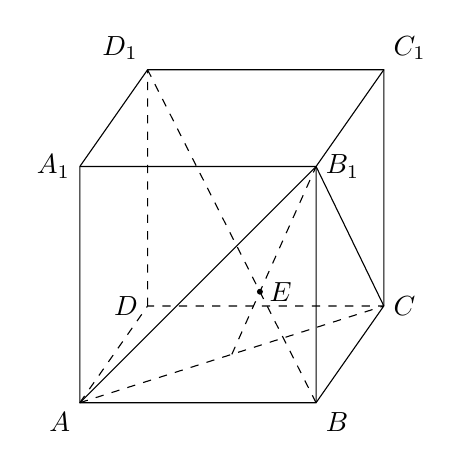
\begin{tikzpicture}[>=latex]
\draw (0,0) node [below left] {$A$} coordinate (A) --++ (3,0) node [below right] {$B$} coordinate (B) --++ (55:{3/2}) node [right] {$C$} coordinate (C)
--++ (0,3) node [above right] {$C_1$} coordinate (C1)
--++ (-3,0) node [above left] {$D_1$} coordinate (D1) --++ (235:{3/2}) node [left] {$A_1$} coordinate (A1) -- cycle;
\draw (A) ++ (3,3) node [right] {$B_1$} coordinate (B1) -- (B) (B1) --++ (55:{3/2}) (B1) --++ (-3,0);
\draw [dashed] (A) --++ (55:{3/2}) node [left] {$D$} coordinate (D) --++ (3,0) (D) --++ (0,3);
\draw (A) -- (B1) -- (C);
\draw [dashed] (A) -- (C) (B) -- (D1) ($(A)!0.5!(C)$) coordinate (O) -- (B1);
\filldraw ($(O)!{1/3}!(B1)$) circle (0.03) node [right] {$E$} coordinate (E);
\end{tikzpicture}
\end{center}
(1) $BD_1\perp$平面$ACB_1$;\\
(2) $|BE|=\dfrac 12|ED_1|$.
\item 在平面上有如下命题: ``若$O$为直线$AB$外的一点, 则点$P$在直线$AB$上的充要条件是: 存在实数$\lambda$、$\mu$, 满足$\overrightarrow{OP}=\lambda \overrightarrow{OA}+\mu \overrightarrow{OB}$, 且$\lambda +\mu=1$.'' 类比此\item 如图, 在正方体$ABCD-A_1B_1C_1D_1$中, $E$、$F$分别是$BB_1$、$D_1B_1$的中点. 求证: $EF\perp$平面$B_1AC$.
\begin{center}
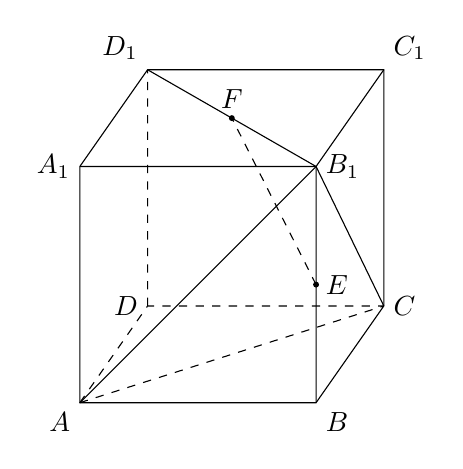
\begin{tikzpicture}[>=latex]
\draw (0,0) node [below left] {$A$} coordinate (A) --++ (3,0) node [below right] {$B$} coordinate (B) --++ (55:{3/2}) node [right] {$C$} coordinate (C)
--++ (0,3) node [above right] {$C_1$} coordinate (C1)
--++ (-3,0) node [above left] {$D_1$} coordinate (D1) --++ (235:{3/2}) node [left] {$A_1$} coordinate (A1) -- cycle;
\draw (A) ++ (3,3) node [right] {$B_1$} coordinate (B1) -- (B) (B1) --++ (55:{3/2}) (B1) --++ (-3,0);
\draw [dashed] (A) --++ (55:{3/2}) node [left] {$D$} coordinate (D) --++ (3,0) (D) --++ (0,3);
\draw (A) -- (B1) -- (C) (B1) -- (D1);
\draw [dashed] (A) -- (C);
\filldraw ($(B)!{1/2}!(B1)$) circle (0.03) node [right] {$E$} coordinate (E);
\filldraw ($(B1)!{1/2}!(D1)$) circle (0.03) node [above] {$F$} coordinate (F);
\draw [dashed] (E) -- (F);
\end{tikzpicture}
\end{center}
\item 在棱长为$1$的正方体$ABCD-A_1B_1C_1D_1$中, $E$、$F$分别是$DD_1$、$DB$的中点, 点$G$在棱$CD$上, $|CG|=\dfrac 14|CD|$, $H$是$C_1G$的中点.\\
(1) 求证: $EF\perp B_1C$;\\
(2) 求$EF$与$C_1G$所成角的余弦值;\\
(3) 求线段$FH$的长.
\item 已知长方体$ABCD-A_1B_1C_1D_1$的棱长$|AB|=14$, $|AD|=6$, $|AA_1|=10$, 以这个长方体的顶点$A$为坐标原点, 分别以射线$AB$、$AD$、$AA_1$为$x$轴、$y$轴、$z$轴的正半轴, 建立空间直角坐标系. 求长方体各顶点的坐标.
\item 已知$PA$垂直于正方形$ABCD$所在的平面, $M$、$N$分别是$AB$、$PC$的中点, 且$|PA|=|AD|$, 分别以射线$AB$、$AD$、$AP$为$x$轴、$y$轴、$z$轴的正半轴, 建立空间直角坐标系. 求向量$\overrightarrow{MN}$、$\overrightarrow{DC}$的坐标表示.
\item 已知$\overrightarrow a=\overrightarrow i+\overrightarrow j-4\overrightarrow k, \overrightarrow b=\overrightarrow i-2\overrightarrow j+2\overrightarrow k$. 求:\\
(1) 向量$\overrightarrow a$与$\overrightarrow b$的夹角的大小;\\
(2) 向量$\overrightarrow a$与$\overrightarrow b$所在直线的夹角的大小.
\item 已知平行四边形$ABCD$中的三个顶点的坐标分别为$A(1, 2, 3)$、$B(2, -1, 5)$与$C(3, 2, -5)$, 求顶点$D$的坐标.
\item 设$\overrightarrow a=(a_1, a_2, a_3)$, $\overrightarrow b=(b_1, b_2, b_3)$, 且$\overrightarrow a\ne \overrightarrow b$. 记$|\overrightarrow a-\overrightarrow b|=m$, 求$\overrightarrow a-\overrightarrow b$与$x$轴正方向向量夹角的余弦值.
\item 在$\triangle ABC$中, 已知$\overrightarrow{AB}=(2, 4, 0)$, $\overrightarrow{BC}=(-1, 3, 0)$. 求$\angle ABC$的大小.
\item 给定空间三点$A(0, 2, 3), B(-2, 1, 6), C(1, -1, 5)$.\\
(1) 求以向量$\overrightarrow{AB}$、$\overrightarrow{AC}$为一组邻边的平行四边形的面积$S$;\\
(2) 若向量$\overrightarrow a$与向量$\overrightarrow{AB}$、$\overrightarrow{AC}$都垂直, 且$|\overrightarrow a|=\sqrt 3$, 求向量$\overrightarrow a$的坐标.
\item 如图, 在直三棱柱$ABC-A_1B_1C_1$中, $|CA|=|CB|=1$,
$\angle BCA=90^\circ$ ,$|AA_1|=2$, $M$、$N$分别是$A_1B_1$、$A_1A$的中点. 建立适当的空间直角坐标系, 解决如下问题:
\begin{center}
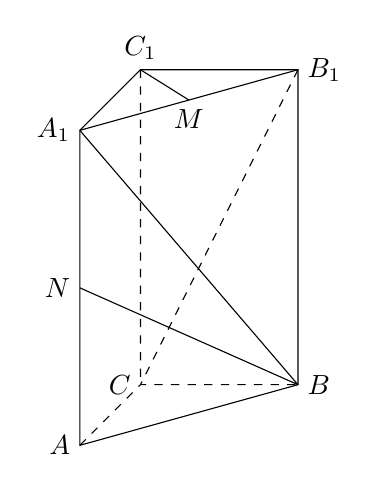
\begin{tikzpicture}[>=latex,scale = 2]
\draw (0,0,0) node [left] {$C$} coordinate (C);
\draw (1,0,0) node [right] {$B$} coordinate (B);
\draw (0,0,1) node [left] {$A$} coordinate (A);
\draw (A) ++ (0,2,0) node [left] {$A_1$} coordinate (A1);
\draw (B) ++ (0,2,0) node [right] {$B_1$} coordinate (B1);
\draw (C) ++ (0,2,0) node [above] {$C_1$} coordinate (C1);
\draw ($(A)!0.5!(A1)$) node [left] {$N$} coordinate (N);
\draw ($(A1)!0.5!(B1)$) node [below] {$M$} coordinate (M);
\draw (C1) -- (M) (A1) -- (B) (N) -- (B);
\draw (A) -- (B) -- (B1) -- (C1) -- (A1) -- cycle;
\draw (A1) -- (B1);
\draw [dashed] (A) -- (C) -- (B) (B1) -- (C) (C1) -- (C);
\end{tikzpicture}
\end{center}
(1) 求$\overrightarrow{BN}$的模;\\
(2) 求$\cos \langle \overrightarrow{BA_1}, \overrightarrow{CB_1}\rangle$;\\
(3) 求证: $A_1B\perp C_1M$.
\item 在正四棱柱$ABCD-A_1B_1C_1D_1$中, $|AA_1|=2|AB|=2$, $E$为$AA_1$的中点. 求异面直线$BE$与$CD_1$所成角的大小.
\item 在正方体$ABCD-A_1B_1C_1D_1$中, $M$、$N$、$P$分别是$CC_1$、$B_1C_1$、$C_1D_1$的中点. 求证: 平面$MNP\parallel$平面$A_1BD$.
\item 在正方体$ABCD-A_1B_1C_1D_1$中, 求$BB_1$与平面$ACD_1$所成角的大小.
\item 如图, 已知正三棱柱$ABC-A_1B_1C_1$的各条棱长均为$a$, $D$是棱$CC_1$的中点. 求证: 平面$AB_1D\perp$平面$ABB_1A_1$.
\begin{center}
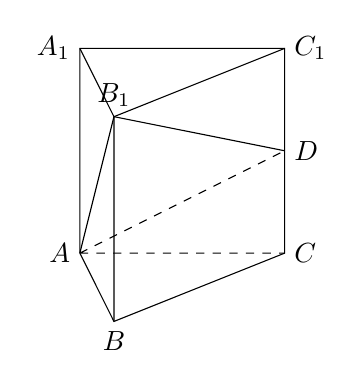
\begin{tikzpicture}[>=latex,scale = 1.3]
\draw (0,0,0) node [left] {$A$} coordinate (A);
\draw (1,0,{sqrt(3)}) node [below] {$B$} coordinate (B);
\draw (2,0,0) node [right] {$C$} coordinate (C);
\draw (A) ++ (0,2,0) node [left] {$A_1$} coordinate (A1);
\draw (B) ++ (0,2,0) node [above] {$B_1$} coordinate (B1);
\draw (C) ++ (0,2,0) node [right] {$C_1$} coordinate (C1);
\draw (B) -- (B1) -- (A1) (B1) -- (C1);
\draw (A) -- (B1) -- ($(C)!0.5!(C1)$) node [right] {$D$} coordinate (D);
\draw (A) -- (B) -- (C) -- (C1) -- (A1) -- cycle;
\draw [dashed] (A) -- (D) (A) -- (C);
\end{tikzpicture}
\end{center}
\item 如图, 已知$P$为平面$ABC$外一点, $AP$、$AB$、$AC$两两互相垂直, 过$AC$的中点$D$作$ED\perp$平面$ABC$, 且$|ED|=1$, $|PA|=2$, $|AC|=2$, 多面体$B-PADE$的体积是$\dfrac {\sqrt 3}3$. 求平面$PBE$与平面$ABC$所成二面角的大小.
\begin{center}
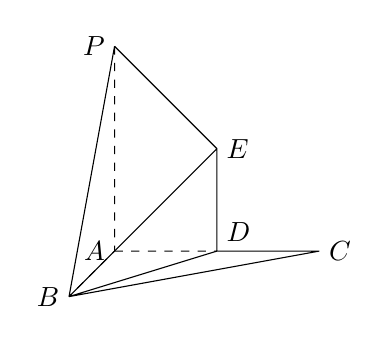
\begin{tikzpicture}[>=latex,scale = 1.3]
\draw (0,0,0) node [left] {$A$} coordinate (A);
\draw (0,0,{2*sqrt(3)/3}) node [left] {$B$} coordinate (B);
\draw (1,0,0) node [above right] {$D$} coordinate (D);
\draw (2,0,0) node [right] {$C$} coordinate (C);
\draw (0,2,0) node [left] {$P$} coordinate (P);
\draw (1,1,0) node [right] {$E$} coordinate (E);
\draw (P) -- (B) (P) -- (E) -- (D) -- (C) (B) -- (E) (B) -- (D) (B) -- (C);
\draw [dashed] (P) -- (A) -- (B) (A) -- (D);
\end{tikzpicture}
\end{center}
\item 如图, 在直棱柱$ABC-A_1B_1C_1$中, $|AA_1|=|AB|=|AC|=2$, $AB\perp AC$, $D$、$E$、$F$分别是$A_1B_1$、$CC_1$、$BC$的中点.
(1) 求$AE$与平面$DEF$所成角的大小;\\
(2) 求$A$到平面$DEF$的距离.
\begin{center}
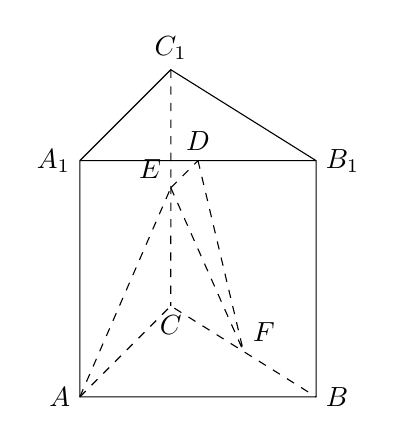
\begin{tikzpicture}[>=latex,scale = 1.5]
\draw (0,0,0) node [left] {$A$} coordinate (A);
\draw (2,0,0) node [right] {$B$} coordinate (B);
\draw (0,0,-2) node [below] {$C$} coordinate (C);
\draw (A) ++ (0,2,0) node [left] {$A_1$} coordinate (A1);
\draw (B) ++ (0,2,0) node [right] {$B_1$} coordinate (B1);
\draw (C) ++ (0,2,0) node [above] {$C_1$} coordinate (C1);
\draw (A) -- (B) -- (B1) -- (C1) -- (A1) -- cycle (A1) -- (B1);
\draw [dashed] (C1) -- (C) (A) -- (C) -- (B);
\draw ($(A1)!0.5!(B1)$) node [above] {$D$} coordinate (D);
\draw ($(C)!0.5!(C1)$)node [above left] {$E$} coordinate (E);
\draw ($(B)!0.5!(C)$) node [above right] {$F$} coordinate (F);
\draw [dashed] (A) -- (E) (E) -- (D) (E) -- (F) (D) -- (F);
\end{tikzpicture}
\end{center}
\item 如图, 在空间四边形$ABCD$中, $|AC|=|AD|$, $\angle BAC=\angle BAD$. 求证: $CD\perp AB$.
\begin{center}
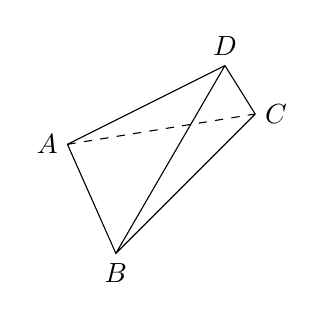
\begin{tikzpicture}[>=latex]
\draw (0,0,0) node [left] {$A$} coordinate (A);
\draw (2,0,-1) node [right] {$C$} coordinate (C);
\draw (2,1,0) node [above] {$D$} coordinate (D);
\draw (A) -- (D) -- (C);
\draw (1,-1,1) node [below] {$B$} coordinate (B);
\draw (A) -- (B) -- (C) (B) -- (D);
\draw [dashed] (A) -- (C); 
\end{tikzpicture}
\end{center}
\item 如图, 在三棱锥$P-ABC$中, $PA\perp$平面$ABC$,$ AB\perp AC$, $|PA|=|AC|=\dfrac 12|AB|$, $M$、$S$分别为$PB$、$BC$的中点, $N$为$AB$上一点, $|BN|=3|NA|$.
\begin{center}
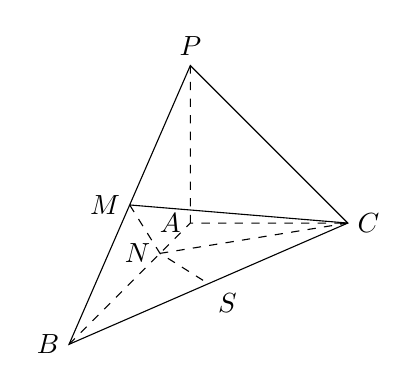
\begin{tikzpicture}[>=latex]
\draw (0,0,0) node [left] {$A$} coordinate (A);
\draw (2,0,0) node [right] {$C$} coordinate (C);
\draw (0,2,0) node [above] {$P$} coordinate (P);
\draw (0,0,4) node [left] {$B$} coordinate (B);
\draw ($(B)!0.5!(C)$) node [below right] {$S$} coordinate (S);
\draw ($(P)!0.5!(B)$) node [left] {$M$} coordinate (M);
\draw ($(A)!0.25!(B)$) node [left] {$N$} coordinate (N);
\draw (B) -- (P) -- (C) -- cycle (C) -- (M);
\draw [dashed] (B) -- (A) -- (C) (A) -- (P) (M) -- (N) -- (S) (N) -- (C);
\end{tikzpicture}
\end{center}
(1) 求证: $CM\perp SN$;\\
(2) 求二面角$PBCA$的大小.
\item 在正方体$ABCD-A_1B_1C_1D_1$中, 设$AB$、$DD_1$的中点分别为$M$、$N$. 求直线$B_1M$与$CN$所成角的大小.
\item 过边长为$1$的正方形$ABCD$的顶点$A$, 作长度为$1$的线段$AE\perp$平面$ABCD$. 求平面$ADE$与平面$BCE$所成二面角的大小.
\item 如图, 在棱长为$1$的正方体$ABCD-A_1B_1C_1D_1$中, $E$、$F$分别为棱$AA_1$、$BB_1$的中点, $G$为棱$A_1B_1$上的一点. 求点$G$到平面$D_1EF$的距离.
\begin{center}
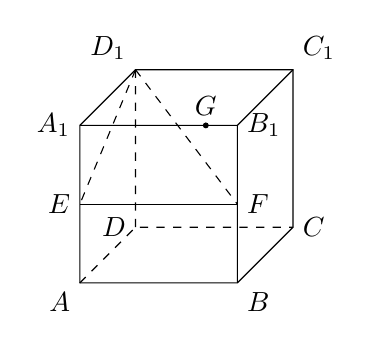
\begin{tikzpicture}[>=latex]
\draw (0,0) node [below left] {$A$} coordinate (A) --++ (2,0) node [below right] {$B$} coordinate (B) --++ (45:{2/2}) node [right] {$C$} coordinate (C)
--++ (0,2) node [above right] {$C_1$} coordinate (C1)
--++ (-2,0) node [above left] {$D_1$} coordinate (D1) --++ (225:{2/2}) node [left] {$A_1$} coordinate (A1) -- cycle;
\draw (A) ++ (2,2) node [right] {$B_1$} coordinate (B1) -- (B) (B1) --++ (45:{2/2}) (B1) --++ (-2,0);
\draw [dashed] (A) --++ (45:{2/2}) node [left] {$D$} coordinate (D) --++ (2,0) (D) --++ (0,2);
\draw ($(A)!0.5!(A1)$)node [left] {$E$} coordinate (E) -- ($(B)!0.5!(B1)$)node [right] {$F$} coordinate (F);
\filldraw ($(A1)!0.8!(B1)$) circle (0.03) node [above] {$G$} coordinate (G);
\draw [dashed] (D1) -- (E) (D1) -- (F);
\end{tikzpicture}
\end{center}
\item 分别求下列两数的等差中项:\\
(1) $8-\dfrac{\sqrt 2}2$与$8+\dfrac{\sqrt 2}2$;\\
(2) $(a+b)^2$与 $(a-b)^2$.
\item 设数列$\{a_n\}$为等差数列, 其公差为$d$.\\
(1) 已知$a_1=2$, $d=3$, 求$a_{10}$;\\
(2) 已知$a_1=3$, $a_n=21, d=2$, 求$n$;\\
(3) 已知$a_1=12$, $a_6=27$, 求$d$;\\
(4) 已知$a_6=9$, $d=-\dfrac 12$, 求$a_1$.
\item 已知数列$\{a_n\}$为等差数列, 其公差为$d$. 求证:对任意给定的正整数$m$、$n$, 都有$a_n=a_m+(n-m)d$.
\item 设数列$\{a_n\}$为等差数列, 其公差为$d$.\\
(1) 已知$a_2=31$, $a_7=76$, 求$a_1$及$d$;\\
(2) 已知$a_1+a_6=12$, $a4=7$, 求$a_9$.
\item 设数列$\{a_n\}$为等差数列, 其公差为$d$, 前$n$项和为$S_n$.\\
(1) 已知$a_1=20$, $a_n=54$, $S_n=999$, 求$d$及$n$;\\
(2) 已知$d=\dfrac 13$, $S_{37}=629$, 求$a_1$及$a_{37}$;\\
(3) 已知$a_1=\dfrac 56$, $d=-\dfrac 16$, $S_n=-5$, 求$n$及$a_n$;\\
(4) 已知$d=2$, $a_{15}=-10$, 求$a_1$及$S_15$.
\item 设数列$\{a_n\}$为等差数列, 其前$n$项和为$S_n$.\\
(1) 已知$a_6=10$, $S_5=5$, 求$S_8$;\\
(2) 已知$S_4=2$, $S_9=-6$, 求$S_{12}$.
\item 设数列$\{a_n\}$为等差数列, 其前$n$项和为$S_n$.\\
(1) 已知$a_4+a_{14}=1$, 求$S_{17}$;\\
(2) 已知$S_{21}=420$, 求$a_{11}$;
(3) 已知$a_1+a_2+a_3=-3$, $a_{18}+a_{19}+a_{20}=6$, 求$S_{20}$;\\
(4) 已知$S_4=2$, $S_8=6$, 求$S_{16}$.
\item 求证: ``$\triangle ABC$三个内角的度数可以构成等差数列''是``$\triangle ABC$中有一个内角为$60^\circ$''的充要条件.
\item 《九章算术》中的``竹九节''问题: 现有一根$9$节的竹子, 自上而下各节的容积成等差数列. 若最上面$4$节的容积共$3$升, 最下面$3$节的容积共$4$升, 则第$5$节的容积为多少升?
\item (1)在等差数列$\{a_n\}$中, 等式$a_n=\dfrac{a_{n-1}+a_{n+1}}2$
($n\ge 2$)是否都成立?\\
(2) 在数列$\{a_n\}$中, 如果对于任意的正整数$n$($n\ge 2$), 都有$a_n=\dfrac{a_{n-1}+a_{n+1}}2$, 那么数列$\{a_n\}$一定是等差数列吗?
\item 在等差数列$\{a_n\}$中, 其前$n$项和为$S_n$. 已知公差$d=24$, $S_{20}=400$.\\
(1) 写出$\displaystyle \sum_{i=1}^{10}a_{2i-1}$的具体展开式, 并求其值;\\
(2) 用求和符号表示$a_2+a_4+a_6+\cdots+a_{20}$, 并求其值.
\item 在等差数列$\{a_n\}$中, 已知$a_1=-3$, $11a_5=5a_8$. 求数列$\{a_n\}$的前$n$项和$S_n$的最小值.
\item 已知等差数列$\{a_n\}$, 其前$n$项和为$S_n$. 若存在两个不相等的正整数$p$和$q$, 满足$S_p=q$, $S_q=p$, 求$S_{p+q}$.
\item 已知一个凸多边形各个内角的度数可以排列成一个公差为$5$的等差数列, 且最小角为$120^\circ$, 该多边形是几边形?
\item 某产品按质量分成$10$个档次, 生产最低档次产品的利润是$8$元/件. 每提高一个档次, 每件产品的利润增加$2$元, 但产量每天减少$3$件. 如果在某段时间内, 最低档次(记作第$1$档次)的产品每天可生产$60$件, 那么在该段时间内, 生产第几档次的产品可获得最大利润?
\item 求下列各组数的等比中项:\\
(1) $\sqrt 3+1$与$\sqrt 3-1$;\\
(2) $a^4+a^2b^2$与$b^4+a^2b^2$($a\ne 0$, $b\ne 0$).
\item 设数列$\{a_n\}$为等比数列, 其公比为$q$.\\
(1) 已知$a_5=8$, $a_8=1$, 求$a_1$、$q$;\\
(2) 已知$a_3=2$, $q=-1$, 求$a_{15}$;\\
(3) 已知$a_4=12$, $a_8=6$, 求$a_{12}$.
\item 已知数列$\{a_n\}$为等比数列, 其公比为$q$. 判断下列数列是否为等比数列. 如果是, 求其公比; 如果不是, 请说明理由.\\
(1) 数列$\{2a_n\}$;\\
(2) 数列$\{a_n+a_{n+1}\}$.
\item 已知数列$\{a_n\}$和数列$\{b_n\}$为项数相同的等比数列, 公比分别为$q_1$和$q_2$. 求证:数列$\{a_nb_n\}$为等比数列, 其公比为$q_1q_2$.
\item 已知直角三角形的斜边长为$c$, 两条直角边长分别为$a$和$b$($a<b$), 且$a, b, c$成等比数列. 求$a:c$的值.
\item 某产品经过$4$次革新后, 成本由原来的$105$元下降到$60$元. 如果这种产品每次革新后成本下降的百分比相同, 那么每次革新后成本下降的百分比是多少? (结果精确到$0.1\%$)
\item 设数列$\{a_n\}$为等比数列, 其公比为$q$, 前$n$项和为$S_n$.\\
(1) 已知$a_1=5$, $q=3$, 求$S_5$;\\
(2) 已知$a_8=\dfrac1{16}$, $q=\dfrac 12$, 求$S_8$;\\
(3) 已知$a_1=-2$, $q=-\dfrac 12$, $a_n= \dfrac 1{1024}$, 求$S_n$;\\
(4) 已知$S_6=\dfrac{189}4$, $q=\dfrac 12$, 求$a_1$.
\item 设等比数列$\{a_n\}$的公比$q<1$, 前$n$项和为$S_n$. 已知$a_3=2$, $S_4=5S_2$, 求数列$\{a_n\}$的通项公式.
\item 一个球从$100\text{m}$高处自由落下, 假设每次着地后又跳回到原高度的一半再落下.\\
(1) 当它第$10$次着地时, 求它经过的总路程;\\
(2) 它可能在某次着地时, 经过的总路程超过$300\text{m}$吗? 如果可能, 请说明是第几次着地首次超过$300\text{m}$; 如果不可能, 请说明理由.
\item 已知$b$是$a$与$c$的等比中项, 且$a$、$b$、$c$同号. 求证: $\dfrac{a+b+c}3,\sqrt{\dfrac{ab+bc+ca}3}, \sqrt[3]{abc}$成等比数列.
\item 已知$a\ne b$, 且$a$、$b$都不为$0$. 设$n$为正整数, 写出$\displaystyle\sum_{i=0}^na^{n-i}b^i$的具体展开式, 并证明$\displaystyle\sum_{i=0}^na^{n-i}b^i=\dfrac{a^{n+1}-b^{n+1}}{a-b}$.
\item 已知对任意给定的正整数$n$, 数列$\{a_n\}$的前$n$项和$S_n=\dfrac{1-q^n}{1-q}$($q\ne 0$且$q\ne 1$). 判断$\{a_n\}$是否为等比数列, 并说明理由.
\item 已知数列$\{a_n\}$为等差数列, 数列$\{bn\}$满足$b_n=(\dfrac 12)^{a_n}$($n$为正整数).\\
(1) 求证: 数列$\{b_n\}$为等比数列;\\
(2) 若$b_1+b_2+b_3=\dfrac{21}8$, $b_1b_2b_3=\dfrac 18$, 求数列$\{a_n\}$的通项公式.
\item 如图, 已知直角三角形$AOB$的两条直角边$AO$和$BO$的长分别为$5$和$12$, 点$O_1$、$O_2$、$\cdots$、$O_n$、$\cdots$在边$OB$上, 半圆$O_1$与$AO$和$AB$所在直线均相切, 半圆$O_2$、$O_3$、$\cdots$、$O_n$、$\cdots$与$AB$所在直线相切, 且与半圆$O_1$、$O_2$、$\cdots$、$O_{n-1}$、$\cdots$分别外切. 设这些半圆的半径分别为$r_1$、$r_2$、$\cdots$、$r_n$、$\cdots$.\\
(1) 求证:数列$\{r_n\}$为等比数列;\\
(2) 求前$n$个半圆弧长的总和$L_n$;\\
(3) 利用前$n$个半圆弧长的总和$L_n$的表达式, 计算$\displaystyle\lim_{n\to+\infty}L_n$.
\begin{center}
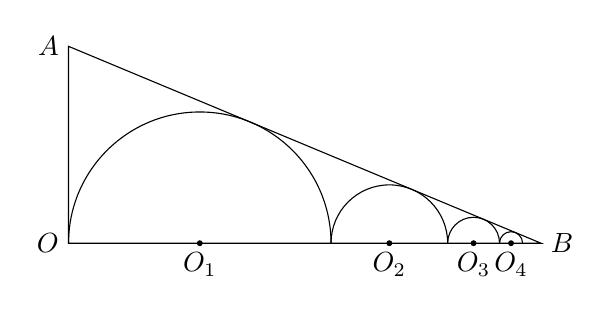
\begin{tikzpicture}[>=latex,scale = 0.5]
\draw (0,5) node [left] {$A$} -- (0,0) node [left] {$O$} -- (12,0) node [right] {$B$}-- cycle;
\draw (0,0) arc (180:0:{10/3}) coordinate (A);
\draw (A) arc (180:0:{10/3*4/9}) coordinate (B);
\draw (B) arc (180:0:{10/3*4/9*4/9}) coordinate (C);
\draw (C) arc (180:0:{10/3*4/9*4/9*4/9}) coordinate (D);
\filldraw ($(0,0)!0.5!(A)$) circle (0.06) node [below] {$O_1$};
\filldraw ($(B)!0.5!(A)$) circle (0.06) node [below] {$O_2$};
\filldraw ($(B)!0.5!(C)$) circle (0.06) node [below] {$O_3$};
\filldraw ($(D)!0.5!(C)$) circle (0.06) node [below] {$O_4$};
\end{tikzpicture}
\end{center}
\item 已知下列数列$\{a_n\}$的通项公式, 写出它的前$4$项.\\
(1) $a_n=n^2-5n$;\\
(2) $a_n=\dfrac{\cos n\pi} 2$.
\item 已知数列$\{a_n\}$的通项公式为$a_n=\dfrac{n^2+n-1}3$, $79\dfrac 23$是否是该数列中的项? 若是, 是第几项?
\item 已知数列$\{a_n\}$的通项公式为$a_n=n^2-8n+5$.\\
(1) 写出这个数列的前$5$项;\\
(2) 这个数列有没有最小项? 如果有, 是第几项? 
\item 已知数列$\{a_n\}$的通项公式为$a_n=(3n-2)(\dfrac 35)^n$, 试问:该数列是否有最大项、最小项? 若有, 分别指出第几项最大、最小; 若没有, 试说明理由.
\item 已知数列$\{a_n\}$的首项$a_1=1$, 且$a_n=2^{n-1}\cdot a_{n-1}$($n\ge 2$). 求数列$\{a_n\}$的通项公式.
\item 已知数列$\{a_n\}$满足$a_1=33$, 且$a_n-a_{n-1}=2(n-1)$($n\ge 2$). 求数列$\{\dfrac{a_n}n\}$的最小项. 
\item 一个正方形被等分成九个相等的小正方形, 将最中间的一个正方形挖掉, 得图\textcircled{1}; 再将剩下的每个正方形都分成九个相等的小正方形, 并将其最中间的一个正方形挖掉, 得图\textcircled{2}; 如此继续下去$\cdots\cdots$\\
(1) 图\textcircled{3}中共挖掉了多少个正方形?\\
(2) 求每次挖掉的正方形个数所构成的数列的一个递推公式.
\begin{center}
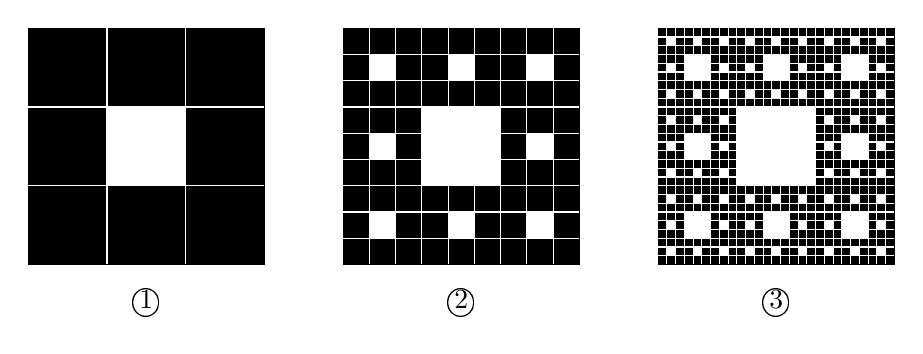
\begin{tikzpicture}[>=latex]
\filldraw (0,0) rectangle (3,3);
\filldraw [white] (1,1) rectangle++ (1,1);
\filldraw (4,0) rectangle (7,3);
\filldraw [white] (5,1) rectangle++ (1,1);
\foreach \i in {{4+1/3},{5+1/3},{6+1/3}} {\foreach \j in {{1/3},{1+1/3},{2+1/3}} {\filldraw [white] (\i,\j) rectangle++ ({1/3},{1/3});};};
\filldraw (8,0) rectangle (11,3);
\filldraw [white] (9,1) rectangle++ (1,1);
\foreach \i in {{8+1/3},{9+1/3},{10+1/3}} {\foreach \j in {{1/3},{1+1/3},{2+1/3}} {\filldraw [white] (\i,\j) rectangle++ ({1/3},{1/3});};};
\foreach \i in {{8+1/9},{8+1/3+1/9},{8+2/3+1/9},{9+1/9},{9+1/3+1/9},{9+2/3+1/9},{10+1/9},{10+1/3+1/9},{10+2/3+1/9}} {\foreach \j in {{1/9},{1/3+1/9},{2/3+1/9},{1+1/9},{1+1/3+1/9},{1+2/3+1/9},{2+1/9},{2+1/3+1/9},{2+2/3+1/9}} {\filldraw [white] (\i,\j) rectangle++ ({1/9},{1/9});};};
\foreach \i in {1,2} {\draw [white] (\i,0) -- (\i,3); \draw [white] (0,\i) -- (3,\i);};
\foreach \i in {1,2,...,8} {\draw [white] ({4+\i/3},0) -- ({4+\i/3},3); \draw [white] (4,{\i/3}) -- (7,{\i/3});};
\foreach \i in {1,2,...,26} {\draw [white] ({8+\i/9},0) -- ({8+\i/9},3); \draw [white] (8,{\i/9}) -- (11,{\i/9});};
\draw (1.5,-0.5) node {\textcircled{1}};
\draw (5.5,-0.5) node {\textcircled{2}};
\draw (9.5,-0.5) node {\textcircled{3}};
\end{tikzpicture}
\end{center}
\item 已知数列$\{a_n\}$的通项公式为$a_n=\dfrac{n-\sqrt {97}}{n-\sqrt {98}}$, 试问: 该数列是否有最大项、最小项? 若有, 分别指出第几项最大、最小; 若没有, 试说明理由.
\item 已知数列$\{a_n\}$的通项公式为$a_n=n^2+\lambda n$, 其中$\lambda$是常数. 若数列$\{a_n\}$为严格增数列, 求$\lambda$的取值范围.
\item 已知数列$\{a_n\}$的前$n$项和为$S_n$, 且$a_1=1$, $a_{n+1}=2S_n$($n$为正整数). 求数列$\{a_n\}$的通项公式.
\item 已知数列$\{a_n\}$的前$n$项和为$S_n=12-12\cdot(\dfrac 23)^n$.\\
(1) 求数列$\{a_n\}$的通项公式;\\
(2) 若数列$\{b_n\}$满足$b_n=(2n-1)a_n$, 问是否存在正整数$m$, 使得$b_m\ge 9$成立, 并说明理由.
\item 某皮革厂第$1$年初有资金$1000$万元, 由于引进了先进的生产设备, 资金年平均增长率可达到$50\%$. 每年年底定额扣除下一年的消费基金后, 将剩余资金投入再生产. 这家皮革厂每年应扣除多少消费基金, 才能实现资金在第$5$年年底扣除消费基金后达到$2000$万元的目标? (结果精确到$1$万元)
\item 用数学归纳法证明$1+a+a^2+\cdots+a^{n+1}=\dfrac{1-a^{n+2}}{1-a}$ ($a\ne 1$, $n$为正整数). 在验证$n=1$等式成立时, 等式左边为\bracket{20}.
\fourch{$1$}{$1+a$}{$1+a+a^2$}{$1+a+a^2+a^3$}
\item 用数学归纳法证明: $1\times 2+2\times 5+\cdots+n(3n-1)=n^2(n+1)$($n$为正整数).
\item 用数学归纳法证明: $\dfrac 1{1\times 3}+ \dfrac 1{3\times 5}+ \dfrac 1{5\times 7}+\cdots+\dfrac 1{(2n-1)(2n+1)}= \dfrac n{2n+1}$($n$为正整数).
\item 已知数列$\{a_n\}$满足$a_1=1$, 设该数列的前$n$项和为$S_n$, 且$S_n, S_{n+1}, 2a_1$成等差数列. 用数学归纳法证明: $S_n=\dfrac{2^n-1}{2^{n-1}}$($n$为正整数).
\item 用数学归纳法证明: $1\cdot n+2\cdot (n-1) +3\cdot (n-2)+\cdots+n\cdot 1=\dfrac 16n(n+1)(n+2)$($n$为正整数).
\item 已知数列$\{a_n\}$满足$a_1=\dfrac 12$, 且对任意正整数$n$, $a_1+a_2+\cdots+a_n=n^2a_n$成立. 试用数学归纳法证明: $a_n=\dfrac1{n(n+1)}$.
\item 设$a_n=1+\dfrac 12+\dfrac 13+\cdots+\dfrac 1n$($n$为正整数), 是否存在一次函数$g(x)=kx+b$, 使得等式$a_1+a_2+a_3+\cdots+a_{n-1}=g(n)(a_n-1)$对大于$1$的正整数$n$都成立? 证明你的结论.




\end{enumerate}

\end{document}